\documentclass{beamer}
\mode<presentation>
\usepackage{amsmath}
\usepackage{amssymb}
\usepackage{bm}
\usepackage{adjustbox}
\usepackage{subcaption}
\usepackage{enumerate}
\usepackage{multicol}
\usepackage{mathtools}
\usepackage{listings}
\usepackage{url}
\def\UrlBreaks{\do\/\do-}
\usetheme{Boadilla}
\usecolortheme{lily}
\setbeamertemplate{footline}
{
  \leavevmode%
  \hbox{%
  \begin{beamercolorbox}[wd=\paperwidth,ht=2.25ex,dp=1ex,right]{author in head/foot}%
    \insertframenumber{} / \inserttotalframenumber\hspace*{2ex} 
  \end{beamercolorbox}}%
  \vskip0pt%
}
\setbeamertemplate{navigation symbols}{}

\providecommand{\nCr}[2]{\,^{#1}C_{#2}}
\providecommand{\nPr}[2]{\,^{#1}P_{#2}}
\providecommand{\mbf}{\mathbf}
\providecommand{\pr}[1]{\ensuremath{\Pr\left(#1\right)}}
\providecommand{\qfunc}[1]{\ensuremath{Q\left(#1\right)}}
\providecommand{\sbrak}[1]{\ensuremath{{}\left[#1\right]}}
\providecommand{\lsbrak}[1]{\ensuremath{{}\left[#1\right.}}
\providecommand{\rsbrak}[1]{\ensuremath{{}\left.#1\right]}}
\providecommand{\brak}[1]{\ensuremath{\left(#1\right)}}
\providecommand{\lbrak}[1]{\ensuremath{\left(#1\right.}}
\providecommand{\rbrak}[1]{\ensuremath{\left.#1\right)}}
\providecommand{\cbrak}[1]{\ensuremath{\left\{#1\right\}}}
\providecommand{\lcbrak}[1]{\ensuremath{\left\{#1\right.}}
\providecommand{\rcbrak}[1]{\ensuremath{\left.#1\right\}}}
\providecommand{\rank}{\text{rank}}
\theoremstyle{remark}
\newtheorem{rem}{Remark}
\newcommand{\sgn}{\mathop{\mathrm{sgn}}}
\providecommand{\abs}[1]{\ensuremath{\left\vert #1 \right\vert}}
\providecommand{\res}[1]{\Res\displaylimits_{#1}} 
\providecommand{\norm}[1]{\lVert#1\rVert}
\providecommand{\mtx}[1]{\mathbf{#1}}
\providecommand{\mean}[1]{\overline{#1}}
\providecommand{\fourier}{\overset{\mathcal{F}}{ \rightleftharpoons}}
\providecommand{\system}{\overset{\mathcal{H}}{ \longleftrightarrow}}
\providecommand{\dec}[2]{\ensuremath{\overset{#1}{\underset{#2}{\gtrless}}}}

% Use your macro for vectors
\renewcommand{\vec}[1]{\begin{pmatrix}#1\end{pmatrix}}

\newenvironment{amatrix}[1]{%
  \left(\begin{array}{@{}*{#1}{c}|c@{}}
}{%
  \end{array}\right)
}

\lstset{
frame=single, 
breaklines=true,
columns=fullflexible
}
\usepackage{listings}
\lstset{
  language=Python,
  basicstyle=\ttfamily\small,
  numbers=left,
  numberstyle=\tiny,
  breaklines=true,
  frame=single
}

\title{Matgeo-2.10.8}
\author{AI25BTECH11019-Menavath Sai Sanjana}

\date{}

\begin{document}

\begin{frame}
\titlepage
\end{frame}

\begin{frame}
\frametitle{Question}

\frametitle{Question}
Let $\vec{b} = 4\hat{i} + 3\hat{j}$ and $\vec{c}$ be two vectors perpendicular to each other in the XY plane. All vectors in the same plane having projections $1$ and $2$ along $\vec{b}$ and $\vec{c}$, respectively, are given by .
\end{frame}

\begin{frame}
\frametitle{Solution}
Consider $\vec{r} = \vec{r_1\\r_2}$, where $r_1$ and $r_2$ are the x- and y-components of the vector we want to find.

\begin{align}
\vec{b} = \vec{4\\3}, \quad
\vec{c} = \vec{x\\y} \text{ (perpendicular to } \vec{b}\text{)}
\end{align}

\begin{align}
\text{Scalar projection on } \vec{b}: \quad 
\frac{\vec{r}^T \vec{b}}{\norm{\vec{b}}} = 1 
\quad \Rightarrow \quad \vec{r}^T \vec{b} = 5
\end{align}

\begin{align}
\text{Since } \vec{c} \perp \vec{b}, \quad 4x + 3y = 0 
\quad \Rightarrow \quad x = -3t, \, y = 4t
\end{align}
     
\begin{align}
\text{Scalar projection on } \vec{c}: \quad
\frac{\vec{r}^T \vec{c}}{\norm{\vec{c}}} = 2 
\quad \Rightarrow \quad \vec{r}^T \vec{c} = 10t
\end{align}
\end{frame}

\begin{frame}
\frametitle{Solution (Continuation)}
\begin{align}
\vec{r}^T \vec{b} &= 4 r_1 + 3 r_2 = 5 \\
\vec{r}^T \vec{c} &= -3 r_1 + 4 r_2 = 10
\end{align}

\begin{align}
\text{Solving the system:} \quad
4 r_1 + 3 r_2 &= 5, \quad -3 r_1 + 4 r_2 = 10
\end{align}

\begin{align}
r_1 &= -\frac{2}{5}, \quad r_2 = \frac{11}{5}
\end{align}
\end{frame}

\begin{frame}
\frametitle{Conclusion}
\noindent\textbf{Conclusion:}  
The required vector is
$
\vec{r} = \vec{-\frac{2}{5}\\ \frac{11}{5}}.
$
\end{frame}


\begin{frame}
\frametitle{Graphical Representation}

\begin{figure}[ht!]
    \centering
    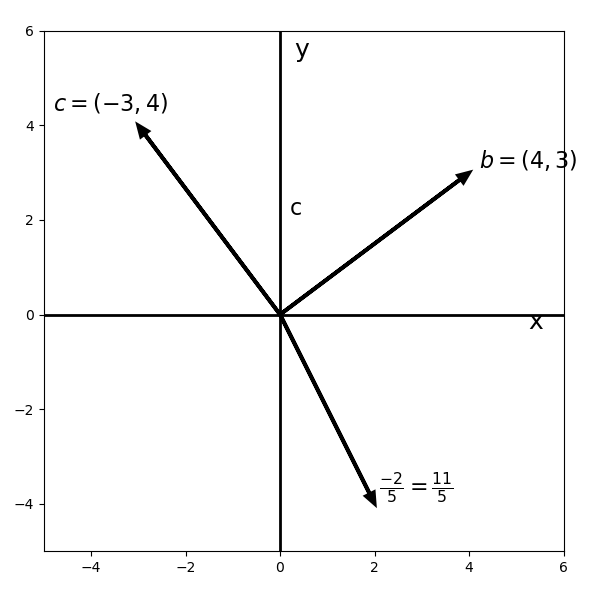
\includegraphics[width=0.7\textwidth]{matgeo-2.10.8.png}
    \caption{}
    \label{fig:1.2.27.jpg}
\end{figure}
\end{frame}

\end{document}

